\documentclass[11pt]{article}
\usepackage[a4paper,margin=1in]{geometry}
\usepackage[T1]{fontenc}
\usepackage{lmodern,microtype}
\usepackage{amsmath,amssymb,amsthm}
\usepackage{booktabs,array,longtable}
\usepackage{xcolor,listings}
\usepackage{enumitem,needspace}
\usepackage{tikz}
\usetikzlibrary{positioning,arrows.meta}
\usepackage[hyphens]{url}
\usepackage[hidelinks]{hyperref}
\usepackage{cleveref}
\hypersetup{pdftitle={Static Object Labelling for Verification: From Ideation to JSOLV and ClangSOLV},
 pdfauthor={Jayanta Majumder and Sambuddha Majumder},
 pdfsubject={Application-owned static evidence, Java and C++ implementations},
 pdfkeywords={static analysis, property tags, JSOLV, ClangSOLV, smart pointers}}
\definecolor{codegray}{gray}{0.96}
\lstset{basicstyle=\ttfamily\small,backgroundcolor=\color{codegray},
 frame=single,framerule=0.2pt,columns=fullflexible,keepspaces=true,
 breaklines=true,showstringspaces=false,tabsize=4}
\newcommand{\jsolv}{\textsc{JSOLV}}
\newcommand{\clangsolv}{ClangSOLV}
\newcommand{\tags}{\mathcal{L}}
\newcommand{\env}{\Gamma}
\newtheorem{proposition}{Proposition}
\newtheorem{definition}{Definition}
\title{Static Object Labelling for Verification:\\
From Semantic Categories and Property-Tag Ideation\\
to JSOLV and ClangSOLV}
\author{Jayanta Majumder \and Sambuddha Majumder}
\date{11 October 2026}
\begin{document}
\maketitle
\begin{abstract}
An ordinary type identifies the kind of a program value, but rarely records
whether that value has been persisted, validated, authenticated, reconciled,
or processed through another required workflow. Encoding every combination
of these independent facts as a nominal type can obscure the domain model
and complicate otherwise ordinary APIs. This paper develops an alternative:
application-owned symbolic labels, checked as a flow-sensitive layer over
ordinary types. It unifies two prior lines of ideation---explicit semantic
categories for legible programming languages, and user-defined static property
tags---with two implemented tools. JSOLV generates Java annotations from a
small configuration and checks their contracts during javac processing.
ClangSOLV generates C++ label declarations and uses a standalone Clang
LibTooling frontend to check contracts before native compilation. Both tools
use independent positive facts, subset requirements, intersection at joins,
and a single-input preservation contract that composes arbitrary label sets.
ClangSOLV additionally implements conservative effect invalidation, structured
loop analysis, explicit proof markers, and pointee labels for standard smart
pointers. We present the motivating philosophy, a common mathematical model,
complete application examples, build integration, diagnostics, implementation
differences, trust assumptions, regression evidence, and a research agenda.
The paper separates implemented contract-flow checking from broader proposed
features such as negative facts, contextual tags, verified postconditions and
heap-sensitive reasoning. Neither implementation is claimed to prove domain
predicates or arbitrary program correctness. Their practical contribution is
to make selected semantic obligations visible and mechanically checkable
without changing the application's ordinary object representation.
\end{abstract}
\tableofcontents
\newpage

\section{Introduction: what an ordinary type leaves unsaid}
A publishing function can accept an \texttt{Article}, a payment function a
\texttt{Payment}, and a numerical routine a \texttt{Matrix}. These types answer
important questions about representation and permitted operations. They do
not normally say whether this particular article was persisted, this payment
authorised, or this matrix checked for positive definiteness. Those facts
often determine whether a call is meaningful even when every conventional
type check succeeds.

Programmers compensate using names, comments, runtime checks, wrapper types,
and informal sequencing rules. A function named \texttt{publishValidated}
signals an intention but cannot by its name prevent an unvalidated argument.
A runtime assertion may catch a violation, but only during an execution that
reaches it. A wrapper such as \texttt{ValidatedArticle} can enforce a useful
construction boundary, but many independent facts produce pressure for many
wrapper combinations and conversions.

The approach studied here retains ordinary domain types while adding a
separate layer of static knowledge. A value can simultaneously have
\texttt{Persisted}, \texttt{Validated}, and \texttt{Authenticated}, without
becoming a new nominal kind of article. A consumer lists the facts it needs;
producer contracts describe what their results establish; a checker follows
the supported value flow and rejects a use lacking required evidence.

This is a synthesis of four local research artifacts. The first argues that
mainstream syntax should reveal materially different semantic roles rather
than encode them all as classes~\cite{roles}. The second proposes a general
static property-tag layer~\cite{ideation}. Two subsequent papers document
Java and C++ implementations~\cite{java-paper,cpp-paper}. Their central
arguments and mechanisms are restated here: no earlier paper is required
to understand the system or reproduce the examples.

\subsection{Contributions and boundaries}
The paper contributes a unified account of five design choices:
\begin{enumerate}[nosep]
\item separate nominal type identity from transient, correctness-relevant facts;
\item let application teams declare their vocabulary without editing analyzers;
\item keep behavioral contracts beside function signatures, rather than in a
second configuration language;
\item compose labels through a small set algebra and explicit preservation;
\item distinguish checked evidence transport from trusted domain semantics.
\end{enumerate}
It also explains why Java and C++ require different engineering compromises.
JSOLV uses native annotation syntax and Maven generation. ClangSOLV uses
declaration macros and a separate compiler-like executable, including a
bounded smart-pointer model. The portable template-based CSOLV alternative
is discussed for context, but this paper's implemented subjects are JSOLV
and ClangSOLV.

``Verification'' here means checking that a requirement follows from the
tool's supported propagation rules and supplied summaries. It does not mean
proving that a database commit occurred, a validator is correct, a credential
is authentic, or a mutable object cannot change elsewhere. A precise account
of these limits is part of the design, not an optional qualification.

\section{Semantic categories and codebase legibility}
\subsection{The many architectural meanings of a class}
Classes in mainstream codebases serve several roles: passive compound data,
encapsulated mutable objects, namespace-like collections of static functions,
service facades, callback objects, policy objects, and wrappers introduced
solely to encode a static condition. Their common syntax is flexible, but a
reader must often reconstruct the intended role from member patterns,
constructors, naming conventions, or documentation.

The earlier semantic-category proposal argues for exposing stable distinctions
when they improve understanding and enable meaningful restrictions. A record
primarily groups data. A stateful object emphasizes identity and invariants.
A module groups declarations without per-instance identity. A callable
emphasizes behavior as a value. A property declaration records knowledge
orthogonal to a nominal type. These categories need not require a new language
all at once; the argument provides a criterion for evaluating their usefulness.

\begin{table}[ht]
\centering\small
\begin{tabular}{>{\raggedright\arraybackslash}p{0.19\linewidth}>{\raggedright\arraybackslash}p{0.35\linewidth}>{\raggedright\arraybackslash}p{0.35\linewidth}}
\toprule
Role & Information made explicit & Possible enforcement benefit\\
\midrule
Record & Data composition & Restricted inheritance and generated structural operations\\
Stateful object & Identity and hidden invariants & Controlled mutation through an interface\\
Module & Grouping without instances & No accidental per-instance state\\
Callable & Behavior and captured context & Explicit capture and invocation rules\\
Static property & Knowledge about a current value & Required evidence at designated uses\\
\bottomrule
\end{tabular}
\caption{Semantic categories motivating the property-label design. These are
conceptual roles, not new declaration kinds implemented by the present tools.}
\end{table}

Naming conventions help but are advisory and locally variable. An explicit
language or tooling category can provide a reliable signal to code browsers,
reviewers and analyzers, and can narrow the legal design space. The benefit
is especially visible under incomplete familiarity: a maintainer entering
a large repository must learn its architecture without reading it linearly.

The philosophy does not require replacing every class. A new category is
worth introducing when its role is frequent, readers benefit from seeing it,
tools can enforce useful restrictions, and the construct removes more
boilerplate than conceptual overhead. The present work applies that threshold
to semantic properties using existing language extension points.

\subsection{Ontology and epistemology}
The distinction can be expressed as
\[
 x:T \qquad\hbox{versus}\qquad x:T\;\{P_1,\ldots,P_k\}.
\]
The first judgment describes what the value is. The second also describes
what is known about it at a program point. An article remains an article
after validation; knowledge of its validity changes. Conversely, a domain
type such as \texttt{AccountId} may deserve nominal identity regardless of
whether its current value has been checked against an account registry.

This distinction also guides API design. A new nominal type is appropriate
when it represents a domain concept, a distinct operation set, or an
encapsulation boundary. A label is appropriate when the same representation
and operations remain useful while selected consumers demand additional
facts. Neither mechanism eliminates the other.

\subsection{Independent facts and nominal proliferation}
With $n$ independent Boolean conditions, up to $2^n$ combinations are
conceptually possible. This does not imply that a wrapper-based program must
declare $2^n$ classes: generic wrappers and phantom types can encode combinations
compactly. It does explain why naming every useful combination is unattractive.
Labels instead represent combinations as sets and keep ordinary APIs usable.

Representation benefits must also be stated carefully. A label layer avoids
introducing a new runtime wrapper representation, but wrapper types do not
necessarily allocate or have measurable runtime overhead. Their principal
tradeoff here is a change to API types and composition, not a universal
performance penalty.

\section{From property-tag ideation to a deliberately small core}
\subsection{The broad proposal}
The ideation paper treats user-defined tags as atomic propositions over
program values. It proposes introduction at proof points, requirements at
consumers, invalidation on changes, and interprocedural summaries. It also
considers definite negative information, predicate-sensitive branches,
parameterized properties, implication hierarchies, linear capabilities,
scoped facts, proof tokens, and interaction with ownership and concurrency.

The central value-centric intuition is that a fact belongs to the current
value or object state, not permanently to an identifier. After
\texttt{x = readOtherValue()}, evidence for the old value does not certify
the replacement. In SSA terminology, the two assignments bind different
value versions. For mutable heap objects, the analogous distinction requires
reasoning about object state and aliases, not merely variable names.

\subsection{Implemented positive evidence}
Both implementations select a smaller fragment: finite sets of independent,
positive, uninterpreted labels. A missing label means \emph{not established
by this analysis}, not \emph{proved false}. There is no built-in implication
from \texttt{Authenticated} to \texttt{Validated}, and no negative requirement
such as \texttt{!Confidential}.

This fragment avoids a logical solver and keeps configuration limited to
names. Even a small core offers a useful workflow guarantee: supported call
sites cannot pass values to designated consumers without evidence for every
listed prerequisite. More ambitious features require new semantics and tests;
they are not implied by the vocabulary's extensibility.

\begin{longtable}{>{\raggedright\arraybackslash}p{0.36\linewidth}>{\raggedright\arraybackslash}p{0.52\linewidth}}
\toprule
Idea & Status in the implemented systems\\\midrule
\endhead
Application-defined positive labels & Implemented in both\\
Requirements and trusted return facts & Implemented in both\\
Single-input, all-label preservation & Implemented in both\\
Branch and conditional intersection & Implemented in both\\
Loop fixed points and reachability & Structured subset in ClangSOLV; restricted handling in JSOLV\\
Explicit establish/require/forget markers & Implemented in ClangSOLV\\
Conservative mutation and effect kills & Implemented in ClangSOLV; not general JSOLV effect analysis\\
Smart-pointer pointee evidence & Implemented bounded subset in ClangSOLV\\
Negative facts and refutation & Proposed only\\
Predicate-dependent validation contracts & Proposed only\\
Context parameters and implication rules & Proposed only\\
Linear labels and scoped capabilities & Proposed only\\
Verified postconditions and proof tokens & Proposed only\\
Precise heap identity and concurrent state & Future work\\
\bottomrule
\caption{The distinction between ideation and delivered behavior.}
\end{longtable}

\subsection{Why vocabulary and behavior belong in different places}
A properties file declares names such as \texttt{Persisted} and
\texttt{Approved}. Function declarations express behavior. This division
avoids a second language of method selectors, wildcard matching, precedence
rules and external contracts that can drift away from code. Extending the
vocabulary remains a simple application task, while establishing or preserving
a property remains a visible API responsibility.

The configuration does not define the truth of a label. An application must
document what \texttt{Persisted} means: inserted in a local store, committed
durably, acknowledged by a remote service, or something else. The analyzer
only transports the corresponding symbol.

\section{Common mathematical model}
\subsection{Label identity and environments}
Let $\tags$ be the finite label vocabulary relevant to a compilation. Labels
have qualified identities; two labels with the same short spelling in
different packages or namespaces are distinct. An environment maps tracked
compiler symbols to sets:
\[
 \env:V\longrightarrow\mathcal{P}(\tags).
\]
An absent binding is equivalent to the empty set. The symbol identity comes
from the compiler, so shadowed variables with identical spelling do not
share evidence.

Expression evaluation computes an evidence set and, where effects are modeled,
an updated environment:
\[
 \mathcal{E}(e,\env)=(S,\env').
\]
This formulation matters for C++: checking an argument and then invoking an
impure function can consume incoming evidence while erasing other facts.
JSOLV implements a less effect-sensitive variant of the same positive-set
idea.

\subsection{Requirements, fresh values and assignment}
For a consumer requiring $R$, with available evidence $S$,
\[
 \operatorname{accept}(R,S)\iff R\subseteq S,
 \qquad\operatorname{missing}(R,S)=R\setminus S.
\]
A fresh ordinary value supplies no labels unless a supported producer contract
or explicit trusted introduction supplies them. Binding a variable records
the right-hand side's evidence. It does not union the old binding's labels
with the new value's labels.

JSOLV usually replaces just the assigned variable's set. ClangSOLV erases the
environment on a write before installing any fresh result evidence on a
supported destination. The latter rule can lose unrelated facts, but prevents
modeled aliases from retaining old evidence across a write.

\subsection{Call contracts and preservation}
Represent a function summary by requirements $R_1,\ldots,R_m$, declared
result labels $A$, and an optional preserved input index $k$. For incoming
argument sets $S_1,\ldots,S_m$, the call requires $R_i\subseteq S_i$ and yields
\[
 S_{\rm result}=
 \begin{cases}
 A\cup S_k,&\text{if preservation is declared},\\
 A,&\text{otherwise}.
 \end{cases}
\]
Indices count explicit arguments from one. Java's \texttt{@PreservesTags}
defaults to one; C++'s \texttt{preserves()} does the same.

Preservation is label-polymorphic: a validator does not need to list every
label an application may someday add. It promises to retain all facts known
on the selected input. The promise concerns the result's properties, not
object identity. Returning the same mutable object is insufficient if the
operation invalidates an input property.

Only one input is selected. Unioning facts from unrelated inputs onto one
output is not generally justified. An authenticated user and a persisted
article do not automatically make an authenticated article; that relationship
needs a truthful domain-specific contract.

\subsection{Joins and short-circuit evaluation}
Facts survive an alternative only when guaranteed on every relevant incoming
path:
\[
 (\env_1\sqcap\env_2)(v)=\env_1(v)\cap\env_2(v).
\]
Conditional expression evidence is likewise the intersection of alternative
results. Short-circuit evaluation joins the path that skips the right operand
with the path that executes it. Union would be incorrect: a label established
on just one branch cannot justify a consumer after the merge.

The two implementations disagree about which paths are considered reachable.
ClangSOLV ends normal flow at supported returns and throws, and propagates
break and continue separately. JSOLV's current scanner does not generally
prune those exits. The set rule is shared; the control-flow approximation is not.

\subsection{A small compositional argument}
\begin{proposition}[Preservation composition]
Suppose three successful producer calls declare result sets $A$, $B$, $C$.
If the second preserves the first result's evidence and the third preserves
the second's, then the final result carries $A\cup B\cup C$ under the supported
call rules.
\end{proposition}
\begin{proof}
The second call yields $B\cup A$. The third yields
$C\cup(B\cup A)=A\cup B\cup C$. No implication between labels or enumeration
of combinations is required.
\end{proof}
This is a statement about evidence propagation, not semantic truth of the
three domain operations. It is useful precisely because the analyzer need
not interpret the labels to check composition.

\subsection{Complexity and termination}
With $n$ labels and $m$ tracked symbols, a conceptual bit-set representation
needs $O(mn)$ bits. Set inclusion, intersection and union are finite operations.
The actual prototypes use ordinary sets of qualified strings rather than a
specialized bit-vector implementation. No measured timing claim follows from
the algebra alone.

A finite domain makes fixed-point analysis feasible, but does not by itself
prove termination of every arbitrary implementation: transfer monotonicity,
iteration order and auxiliary state also matter. ClangSOLV uses descending
structured-loop iterations with a 1024-pass safety limit. A future general
worklist engine should state and test its convergence assumptions explicitly.

\section{A running publishing example}
Let an article pass through three stages. Persistence establishes
\texttt{Persisted}; validation establishes \texttt{Validated} while retaining
existing facts; authentication establishes \texttt{Authenticated} while
retaining them. Publication demands all three.

\begin{figure}[ht]
\centering
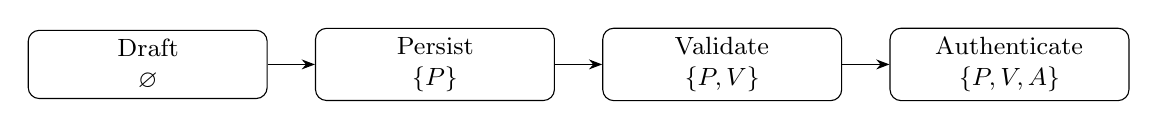
\begin{tikzpicture}[node distance=6mm and 6mm,
 box/.style={draw,rounded corners,align=center,font=\small,text width=28mm},
 >=Stealth]
\node[box] (d) {Draft\\$\varnothing$};
\node[box,right=of d] (p) {Persist\\$\{P\}$};
\node[box,right=of p] (v) {Validate\\$\{P,V\}$};
\node[box,right=of v] (a) {Authenticate\\$\{P,V,A\}$};
\draw[->] (d)--(p);\draw[->] (p)--(v);\draw[->] (v)--(a);
\end{tikzpicture}
\caption{Ordinary domain objects with accumulating evidence. Publication requires
the final set; the letters abbreviate the three independent labels.}
\end{figure}

The example concerns an application's chosen authentication guarantee. It
does not prescribe a security protocol. In particular, a Boolean label cannot
encode a principal, article version, expiry time and policy automatically.
An application may place that context in immutable domain data or use a
more explicit label such as \texttt{DemoAuthorAuthenticated}; parametric
labels remain future work.

\section{JSOLV: architecture and configurable annotations}
\subsection{Components and naming}
JSOLV expands to \emph{Java Static Object Labelling for Verification}.
The repository contains a Maven reactor with annotations, checker, generator
plugin and demo modules, plus an independently built application. The shared
support package is \texttt{org.jsolv}; the processor is
\texttt{org.jsolv.checker.JsolvProcessor}. Version \texttt{1.0-SNAPSHOT}
denotes local development artifacts, not an assertion of Maven Central publication.

An application vocabulary is configured as follows:
\Needspace{5\baselineskip}
\begin{lstlisting}
# jsolv.properties, beside the application's pom.xml
package=example.tags
labels=Persisted, Validated, Authenticated, Approved
\end{lstlisting}
The UTF-8 Java-properties format supports comments and continuations. Exactly
two keys are accepted. Missing keys, unknown keys, duplicates, invalid
identifiers, keywords and malformed label lists fail generation. Application
programmers add a name and rebuild; no checker registry changes.

\subsection{The marker protocol}
Each generated annotation has the following shape:
\Needspace{12\baselineskip}
\begin{lstlisting}[language=Java]
package example.tags;

@org.jsolv.StaticTag
@java.lang.annotation.Retention(
    java.lang.annotation.RetentionPolicy.CLASS)
@java.lang.annotation.Target({
    java.lang.annotation.ElementType.TYPE_USE,
    java.lang.annotation.ElementType.PARAMETER,
    java.lang.annotation.ElementType.METHOD})
public @interface Validated {}
\end{lstlisting}
The Java language provides annotation declarations and their use sites
\cite{jls}; JSOLV assigns the custom flow semantics. Recognition depends on
the \texttt{@StaticTag} meta-annotation, not a package naming convention.
Support annotation names are fully qualified in generated files, avoiding
collisions when an application chooses a label named \texttt{Target}.

CLASS retention permits contracts to be distributed in compiled libraries.
METHOD targeting is deliberate: the checker reads method declaration metadata
as well as return-type metadata, a practical route for ordinary return
annotation placement across the tested JDK 17 compilation boundaries. This
does not claim complete support for every possible nested type-use placement.

The preservation annotation is shared rather than generated per application:
\Needspace{7\baselineskip}
\begin{lstlisting}[language=Java]
@Target(ElementType.METHOD)
@Retention(RetentionPolicy.CLASS)
public @interface PreservesTags {
    int value() default 1;
}
\end{lstlisting}
Imports for \texttt{Target}, \texttt{Retention} and their enums are assumed
in this support-definition excerpt.

\subsection{Generation before checking}
The Maven plugin's \texttt{generate} goal runs in \texttt{generate-sources},
before compilation in the lifecycle~\cite{maven}. It registers a dedicated
generated source root. javac consequently resolves generated annotations
normally before the checker examines their uses.

Combining first-round generation and checking in one processor would introduce
unresolved-import and processing-round complications. Separating vocabulary
generation is simpler and makes failure behavior clearer. The generator
validates before changing output, preserves unchanged timestamps, and removes
obsolete owned generated sources without deleting an arbitrary directory.
Handwritten files are not silently overwritten.

\begin{figure}[ht]
\centering
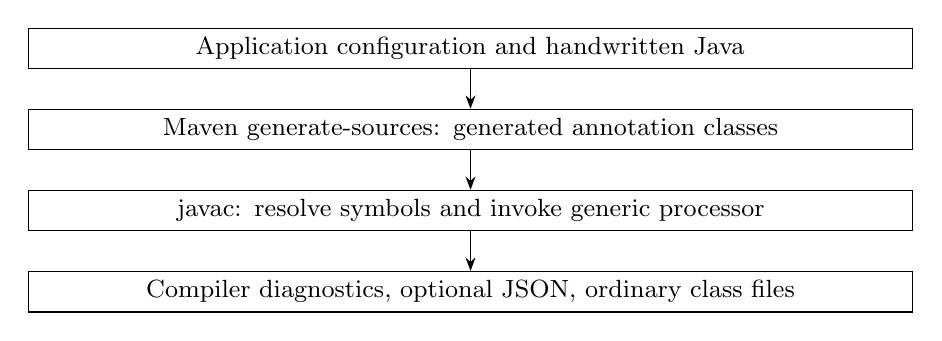
\begin{tikzpicture}[node distance=5mm,
 box/.style={draw,align=center,text width=110mm,font=\small},>=Stealth]
\node[box] (c) {Application configuration and handwritten Java};
\node[box,below=of c] (g) {Maven generate-sources: generated annotation classes};
\node[box,below=of g] (j) {javac: resolve symbols and invoke generic processor};
\node[box,below=of j] (r) {Compiler diagnostics, optional JSON, ordinary class files};
\draw[->](c)--(g);\draw[->](g)--(j);\draw[->](j)--(r);
\end{tikzpicture}
\caption{JSOLV's integration with the ordinary Java build.}
\end{figure}

\section{A complete Java application}
The following class assumes the generated \texttt{example.tags} vocabulary.
The in-memory store and demo credential make domain behavior concrete without
claiming durable persistence or production authentication.
\Needspace{12\baselineskip}
\begin{lstlisting}[language=Java,label=lst:java-core]
import example.tags.*;
import org.jsolv.PreservesTags;
import java.util.ArrayList;
import java.util.List;

public final class PaperWorkflow {
    record Article(String title) {}
    private static final List<Article> STORE = new ArrayList<>();

    static @Persisted Article persist(Article article) {
        STORE.add(article);
        return article;
    }

    @PreservesTags
    static @Validated Article validate(Article article) {
        if (article.title() == null || article.title().isBlank())
            throw new IllegalArgumentException("empty title");
        return article;
    }

    @PreservesTags
    static @Authenticated Article authenticate(
            Article article, String credential) {
        if (!"demo-author".equals(credential))
            throw new IllegalArgumentException("bad demo credential");
        return article;
    }

    static void publish(
            @Persisted @Validated @Authenticated Article article) {
        System.out.println("Published: " + article.title());
    }

    public static void main(String[] args) {
        Article draft = new Article("One type, several facts");
        Article saved = persist(draft);
        Article checked = validate(saved);
        Article ready = authenticate(checked, "demo-author");
        publish(ready);
        publish(authenticate(validate(persist(draft)), "demo-author"));
    }
}
\end{lstlisting}
Each successful return is a trusted postcondition. A bug that removes the
validation check does not automatically make JSOLV reject the method's
\texttt{@Validated} declaration. The checker analyzes calls in the method,
but does not verify its promised return predicates.

\subsection{Rejected calls and local obligations}
In the same class, these additional statements are rejected:
\Needspace{6\baselineskip}
\begin{lstlisting}[language=Java]
publish(draft);                         // no required evidence
publish(validate(persist(draft)));      // missing Authenticated
@Persisted Article forged = draft;     // local annotation is a requirement
publish((@Persisted Article) draft);    // cast does not introduce evidence
\end{lstlisting}
Local annotations impose requirements on their initializer and later
assignments. They do not turn an assertion into a proof. An ordinary
unannotated transformation supplies no result evidence even if its body
returns its input, unless a preservation summary says otherwise.

\subsection{Preservation from another argument}
\Needspace{6\baselineskip}
\begin{lstlisting}[language=Java]
@PreservesTags(2)
static @Validated Article chooseSecond(Article ignored, Article article) {
    return validate(article);
}
\end{lstlisting}
The result retains facts from the second argument. Java validates the
preservation index on source declarations: it must name a valid, non-varargs
parameter and the return must be non-void. The current Java checker does not
enforce the C++ implementation's same-domain-type preservation restriction.
An application must therefore be particularly careful not to transfer
unrelated predicates across types through an untruthful summary.

\subsection{Branches}
\Needspace{7\baselineskip}
\begin{lstlisting}[language=Java]
Article chosen;
if (args.length > 0) chosen = checked;
else chosen = saved;
@Persisted Article common = chosen;     // accepted
// @Validated Article tooStrong = chosen; // rejected
\end{lstlisting}
Only persistence is common to both assignments. A branch followed by an
early return may still be conservatively included by JSOLV, because the
current scanner does not model normal-path reachability fully.

\section{Java build setup and separate compilation}
Install the tools once, then compile the independent example:
\Needspace{4\baselineskip}
\begin{lstlisting}
mvn -f pom.xml clean install
mvn -f example-app/pom.xml clean compile
\end{lstlisting}
The tested baseline recorded by the Java artifact is JDK 17.0.12 and Maven
3.9.11. A JDK is required, including the compiler used by compilation tests.
Teams can deploy the artifacts to their own repository so application
programmers need not rebuild the tooling to add a label.

A consumer depends on the support annotations:
\Needspace{7\baselineskip}
\begin{lstlisting}[language=XML]
<dependency>
  <groupId>org.jsolv</groupId>
  <artifactId>jsolv-annotations</artifactId>
  <version>1.0-SNAPSHOT</version>
</dependency>
\end{lstlisting}
Within \texttt{build/plugins}, generation and checking are configured as follows:
\Needspace{12\baselineskip}
\begin{lstlisting}[language=XML]
<plugin>
  <groupId>org.jsolv</groupId>
  <artifactId>jsolv-maven-plugin</artifactId>
  <version>1.0-SNAPSHOT</version>
  <executions>
    <execution><goals><goal>generate</goal></goals></execution>
  </executions>
</plugin>
<plugin>
  <groupId>org.apache.maven.plugins</groupId>
  <artifactId>maven-compiler-plugin</artifactId>
  <version>3.13.0</version>
  <configuration>
    <release>17</release>
    <proc>full</proc>
    <annotationProcessorPaths>
      <path>
        <groupId>org.jsolv</groupId>
        <artifactId>jsolv-checker</artifactId>
        <version>1.0-SNAPSHOT</version>
      </path>
    </annotationProcessorPaths>
    <compilerArgs>
      <arg>-Ajsolv.report=${project.build.directory}/jsolv-report.json</arg>
    </compilerArgs>
  </configuration>
</plugin>
\end{lstlisting}
Explicit processing makes the build contract visible. The optional report
argument can be omitted. The generator can be configured with a different
\texttt{configFile} or \texttt{outputDirectory}; \texttt{-Djsolv.config=...}
also selects a config file.

Use lifecycle commands such as \texttt{mvn compile}, rather than invoking
\texttt{compiler:compile} directly and skipping generation. An IDE may need
\texttt{mvn generate-sources} and a Maven reimport before resolving newly
generated annotations. After deleting or renaming a label, use a clean build:
removing its generated source need not remove an old compiled class file.

For several application modules, generate the vocabulary once in an
application-owned labels JAR. Consumers depend on it and activate the checker;
they need no duplicate configuration registry. Qualified identities, metadata
retention and compilation-boundary tests support that deployment pattern.

\section{How JSOLV checks Java source}
The processor uses compiler trees and language-model elements through the
JDK \texttt{Trees} bridge~\cite{trees}. It recognizes all annotation types,
selects those marked as static tags, and returns false from processing so
other processors' annotations are not claimed.

Each method begins with its parameters' required label sets. Expression
evaluation handles identifiers, assignments, casts, calls and conditional
expressions, recursively checking nested calls and constructor arguments.
Sets are copied as immutable binding evidence. Expanded varargs arguments
are checked individually; array and component qualifier flow is not a
general feature.

For loops, try statements and switches, potentially assigned variables
are forgotten and branches are checked without deriving general post-statement
facts. This policy is not a full CFG fixed-point analysis. Lambda bodies
start their own environments with parameter contracts; captured locals are
unknown. Fields and array elements provide no tracked value evidence.
Nested generic qualifiers, override compatibility, receiver contracts,
method references and whole-program summaries are outside the implemented
model.

Most importantly, JSOLV does not perform general alias mutation or method
effect invalidation. If an unannotated mutator changes an object denoted by
a labelled binding, the existing binding's evidence can remain. This is
a real limitation: the tool should be used for disciplined immutable or
snapshot-like workflows, rather than advertised as sound for arbitrary
mutable Java programs.

\section{ClangSOLV: a standalone C++ checking frontend}
\subsection{Why a frontend rather than only a template library}
C++ can encode labels in template types, but that changes the types carried
through APIs. A separate portable CSOLV library explores that approach.
ClangSOLV instead aims for JSOLV-like use of ordinary objects, declarations,
assignments and control flow, with evidence managed by a checker.

Clang LibTooling provides infrastructure for standalone compiler-based
tools~\cite{libtooling}. ClangSOLV links its AST, frontend and analysis
libraries, invokes semantic parsing, and inspects resolved declarations.
It is not a textual macro scanner, a compiler fork, or an AST-dumping
subprocess. The executable checks source and reports errors; a native
compiler separately produces the executable.

The frontend validates that Clang can construct a CFG for each checked
function, but its transfer engine follows a supported structured-AST subset.
It is not a general CFG-element solver and does not use Clang's general
flow-sensitive framework. This distinction explains the explicit rejection
of unsupported control-flow constructs.

\subsection{Configuration and generated label types}
\Needspace{5\baselineskip}
\begin{lstlisting}
# clangsolv.properties
namespace=example::tags
labels=Persisted, Validated, Authenticated, Approved
\end{lstlisting}
A Python generator emits a header containing empty record declarations:
\Needspace{8\baselineskip}
\begin{lstlisting}[language=C++]
#include <clangsolv/annotations.hpp>
namespace example::tags {
struct CLANGSOLV_ANNOTATE("clangsolv.label") Persisted {};
struct CLANGSOLV_ANNOTATE("clangsolv.label") Validated {};
// Other configured labels have the same form.
}
\end{lstlisting}
The records identify propositions; applications need not instantiate them.
Macros stringify label names and the analyzer resolves them against qualified
registered records. A short name is accepted only when unambiguous.

The C++ configuration deliberately implements a smaller properties-like
format than Java's. Blank lines and full-line comments are supported, but
Java continuation/escape semantics and inline comments are not. Unknown
keys, duplicates, keywords and invalid identifiers fail generation. Similar
looking config files should not be assumed to have identical parsing rules.

\subsection{Readable public contracts}
\begin{longtable}{>{\raggedright\arraybackslash}p{0.30\linewidth}>{\raggedright\arraybackslash}p{0.58\linewidth}}
\toprule
Syntax & Contract meaning\\\midrule
\endhead
\texttt{returns(L...)} & Successful result establishes the listed labels\\
\texttt{needs(L...)} & Parameter requires every listed label\\
\texttt{preserves()} & Result retains all known labels of explicit argument one\\
\texttt{preserves(k)} & Same rule for explicit argument k, indexed from one\\
\texttt{readonly} & Trusted promise that the call preserves the caller's tracked evidence\\
\bottomrule
\caption{ClangSOLV's deliberately short, unprefixed contract interface.}
\end{longtable}
The name \texttt{needs} leaves the C++20 \texttt{requires} keyword available.
The examples and supplied helper use C++17. The contract macros expand to
Clang annotation attributes during checking; non-Clang native compilation
erases those annotations. The attribute spelling uses familiar C++ attribute
syntax, but \texttt{clang::annotate} and its custom semantics are not a
standard C++ verification feature.

The empty preservation macro argument emits an empty annotation payload;
the checker interprets it as one. This keeps defaulting out of complicated
preprocessor argument-count logic. Explicit invalid indices still fail.
Contracts on public declarations govern calls and definitions across
redeclarations. The checker does not infer implementations across translation
units or prove these summaries.

\section{A complete C++ application}
Generate \texttt{clangsolv\_labels.hpp} from the configuration above and compile
the following single translation unit. Its domain behavior mirrors the Java
example while making the separate effect promise visible.
\Needspace{12\baselineskip}
\begin{lstlisting}[language=C++,label=lst:cpp-core]
#include <clangsolv_labels.hpp>
#include <iostream>
#include <stdexcept>
#include <string>
#include <vector>

namespace example {
struct Article { std::string title; };
std::vector<Article> store;

returns(Persisted) Article persist(Article article);
readonly returns(Validated) preserves()
Article validate(const Article& article);
readonly returns(Authenticated) preserves()
Article authenticate(const Article& article, const std::string& credential);
readonly void publish(
    needs(Persisted, Validated, Authenticated) const Article& article);

Article persist(Article article) {
    store.push_back(article);
    return article;
}
Article validate(const Article& article) {
    if (article.title.empty())
        throw std::invalid_argument("empty title");
    return article;
}
Article authenticate(const Article& article, const std::string& credential) {
    if (credential != "demo-author")
        throw std::invalid_argument("bad demo credential");
    return article;
}
void publish(const Article& article) {
    std::cout << "Published: " << article.title << '\n';
}
}

int main(int argc, char**) {
    using namespace example;
    using namespace example::tags;
    Article chosen;
    const std::string credential="demo-author";
    const auto saved=persist(Article{"One type, several facts"});
    const auto checked=validate(saved);
    const auto ready=authenticate(checked,credential);
    publish(ready);

    if (argc>1) chosen=checked;
    else chosen=saved;
    clangsolv::require<Persisted>(chosen);
    const auto checkedAgain=validate(chosen);
    const auto readyAgain=authenticate(checkedAgain,credential);
    publish(readyAgain);
}
\end{lstlisting}
Raw storage and the credential are constructed before evidence is gathered.
Unknown nontrivial constructor effects can otherwise erase earlier facts.
The explicit temporaries also avoid unsupported side-effecting multi-argument
evaluation patterns.

The output function may truthfully be \texttt{readonly} even though it performs
I/O: the contract means preserving tracked evidence, not mathematical purity.
Persistence is not declared readonly. Its call erases previous evidence
after checking inputs and capturing the contracted result, which can still
establish fresh persistence evidence.

\subsection{Rejected uses}
The following statements, inserted at suitable points after their operands
are declared, illustrate missing evidence:
\Needspace{6\baselineskip}
\begin{lstlisting}[language=C++]
publish(saved);                // missing Validated and Authenticated
publish(checked);              // missing Authenticated
// after chosen's branch join:
clangsolv::require<Validated>(chosen); // not common to both paths
\end{lstlisting}
A member write such as \texttt{chosen.title = "changed"} erases the environment.
It cannot retain a stale validation fact merely because the variable keeps
its name.

\subsection{Explicit markers}
The support library supplies runtime no-op templates:
\Needspace{6\baselineskip}
\begin{lstlisting}[language=C++]
clangsolv::establish<example::tags::Approved>(chosen);
clangsolv::require<example::tags::Approved>(chosen);
clangsolv::forget<example::tags::Approved>(chosen);
clangsolv::forget(chosen);
\end{lstlisting}
Establishment is an explicit trusted assertion, suitable only after a
real application proof point. It unions facts on its named target. Requiring
checks a subset. Forgetting removes chosen facts or all target facts; the
current alias-safe policy also erases other variables' evidence before
retaining any unforgotten facts on the target.

Targets must be named automatic values, supported references or smart
pointers. Global storage and static local storage, unnamed expressions and raw pointers
are not supported marker targets. Label template arguments must be registered
label types. These templates allocate no label storage and do not validate
the object at runtime. In an unoptimized build, no-op calls may still appear;
the claim is no runtime label representation, not a benchmarked zero instruction
cost under every compiler setting.

\section{C++ effects, aliases and structured flow}
\subsection{Invalidation as the conservative default}
After a non-readonly call, the environment is cleared. Requirements are
checked and result evidence captured first. Writes, increments, compound
assignments, address taking and escapes also clear evidence. A supported
plain assignment can then bind fresh right-hand-side evidence on its
destination. Member reads do not inherit all labels on their containing object.

Direct references initialized from a named variable share its evidence
binding. More complex borrowed expressions can have independent conservative
bindings; writes and unknown effects still clear them. This policy avoids
pretending to have a precise points-to analysis. Its cost is rejection of
some safe programs, including ones that mutate an unrelated counter.

Defaulted value copy/move operations retain evidence under a semantic-fidelity
assumption. Nontrivial defaulted copies can invoke member operations, so other
evidence is conservatively erased. Custom constructors do not implicitly
transfer tags. Moves erase incoming evidence before transferring the captured
snapshot. Dangerous reinterpretation and const-removal casts reject checking;
ordinary type-changing casts do not manufacture evidence.

\subsection{Loops and reachable exits}
For a while/for loop with entry environment $E$, the header iteration has
the conceptual form
\[
 H_{i+1}=E\sqcap\operatorname{Back}(H_i).
\]
The back edge includes normal and continue paths and appropriate condition
and increment effects. Break environments contribute to exits. The zero-iteration
path matters for while/for; a do loop runs at least once. Supported returns
and standalone throws terminate the current normal path.

Exploratory fixed-point passes suppress diagnostics; checks are emitted at
the stable state. A finite safety bound rejects unexpected nonconvergence.
The analysis is flow-sensitive, but not a predicate solver: it does not
automatically infer a user label from an arbitrary Boolean validator or
prune all branches with literal conditions.

\subsection{Unsupported syntax and evaluation order}
The frontend rejects switch, goto, range-for, try/catch, coroutines, lambdas,
indirect calls, virtual dispatch, loop condition declarations, dangerous
casts and unmodeled AST expressions. Custom-destructor value constructions
are rejected when visible. This is not complete cleanup analysis for nested
library-managed objects.

C++ argument ordering needs care. Multiple side-effecting arguments,
side-effecting multi-argument contract calls and certain unsequenced binary
patterns are rejected rather than checked using an assumed order. Bind
intermediate results first. Member-operator contracts count explicit
parameters, with Clang's implicit receiver accounted for separately.

Available nondependent user functions and instantiated templates are checked;
uninstantiated dependent bodies are deferred. System-header implementations
are opaque boundaries. Unsupported constructs result in diagnostics rather
than an implied promise of general C++ coverage.

\section{Smart pointers: labels belong to the pointee}
\subsection{The semantic choice}
For \texttt{shared\_ptr<Article>} or \texttt{unique\_ptr<Article>},
\texttt{Validated} should describe the managed article, not the ownership
wrapper. The implementation therefore recognizes the semantic standard-library
template specialization and normalizes its label domain to the pointee type.
Application type aliases are recognized without relying on source spelling.

This keeps ordinary API types:
\Needspace{7\baselineskip}
\begin{lstlisting}[language=C++]
returns(Persisted) std::shared_ptr<Article> persistShared(Article draft);
readonly returns(Validated) preserves()
std::shared_ptr<Article> validateShared(
    const std::shared_ptr<Article>& article);
readonly void inspect(needs(Persisted, Validated) const Article& article);
\end{lstlisting}
No \texttt{tagged<Article,...>} wrapper is inserted between the angle brackets.
C++ declaration attributes do not supply Java's arbitrary type-use annotation
model; the pointee meaning is assigned by ClangSOLV to the declared contract.

\subsection{Copies, moves and dereferencing}
The following fragment is accepted with truthful producer contracts:
\Needspace{7\baselineskip}
\begin{lstlisting}[language=C++]
auto saved=persistShared(Article{"Managed object"});
auto checked=validateShared(saved);
auto alias=checked;
inspect(*alias);
clangsolv::require<example::tags::Validated>(alias);
\end{lstlisting}
Both dereference and arrow operations transfer known pointee evidence.
A shared-pointer copy inherits the evidence known on its source at the copy.
Unique-pointer moves transfer the captured evidence to the destination and
erase source evidence; other facts are conservatively erased too.

\Needspace{8\baselineskip}
\begin{lstlisting}[language=C++]
auto owner=std::make_unique<Article>(Article{"Exclusive ownership"});
// Trusted assertion after an actual application-specific check:
clangsolv::establish<example::tags::Validated>(owner);
auto moved=std::move(owner);
clangsolv::require<example::tags::Validated>(moved); // accepted
// require<Validated>(owner) would be rejected
\end{lstlisting}
Explicit rvalue-reference casts followed by unique-pointer construction also
invalidate the source; transfer is not limited to the spelling \texttt{std::move}.

\subsection{Snapshot evidence instead of a heap graph}
The implementation deliberately copies evidence snapshots rather than
recording precise allocation identity. This makes the specification small:
copies can retain current knowledge, and modeled potentially invalidating
operations erase all knowledge that might be stale.

Mutation through an alias, reset, swap, assignment, get, release and unknown
calls clear the environment, including evidence on copied handles and borrowed
references. Smart-pointer assignment currently restores no destination facts;
initialization from a producer is preferred. Forgetting also clears other
bindings, covering revocation through a copied handle.

\Needspace{6\baselineskip}
\begin{lstlisting}[language=C++]
auto p=persistShared(Article{"Example"});
auto q=p;
q->title="replacement";
// A requirement for Persisted on *p now fails conservatively.
\end{lstlisting}
The policy can discard facts that remain true at runtime. For example,
resetting one shared owner need not invalidate the article owned by another,
but the checker forgets evidence rather than reasoning about that allocation.
Conversely, labels established on one handle after an earlier copy do not
automatically appear on that copy. Establish first and then copy, or use the
explicitly labelled handle.

Preservation compares pointee domain types, ignoring outer ownership wrappers
and const qualification. It promises facts on the result, not that the result
aliases an input. This prevents a preservation summary from being misread as
an allocation-identity proof.

\subsection{Ownership and lifetime boundaries}
Supported ownership is \texttt{shared\_ptr<T>} and \texttt{unique\_ptr<T>}
with the default deleter, for an ordinary single pointee. Arrays, nested
pointer pointees, custom unique deleters, raw-pointer adoption and converting
ownership constructors are rejected. Use make\_shared, make\_unique or
trusted contracted factories. Const observers such as Boolean conversion,
use\_count and unique preserve evidence but supply no labels.

A default or empty pointer has no evidence. A trusted establishment or return
contract describing a pointee must promise that a live managed object exists
and satisfies the predicates. There is no independent nullness, lifetime or
borrow checker. Visible user-defined pointee destructors are rejected;
contracted factories must not hide deleter effects that invalidate other
tracked objects. Hidden custom shared deleters, external aliases, concurrency
and complete destruction analysis remain outside this sequential model.
Raw-pointer contracts remain unsupported. These restrictions are important
when interpreting ``supports smart pointers'': the tool supports a bounded
evidence-flow discipline, not every C++ ownership operation.

\section{C++ build integration and reproducible use}
Building the frontend requires matching LLVM/Clang development headers,
libraries and CMake exports, not only a compiler executable. The tested
installation is LLVM/Clang 19.1.0 with MSVC 19.44 on Windows. LLVM/Clang 18+
is an intended API range, not a validated compatibility matrix. CMake 3.20+
and Python 3.10+ are the documented build baseline.

\Needspace{5\baselineskip}
\begin{lstlisting}
cmake -S development_tools/clangsolv -B build/checker -DLLVM_DIR=/llvm/lib/cmake/llvm -DClang_DIR=/llvm/lib/cmake/clang
cmake --build build/checker --config Release
ctest --test-dir build/checker -C Release --output-on-failure
\end{lstlisting}
Use actual package locations. Multi-configuration builds commonly place the
executable in \texttt{Release/clangsolv.exe}; single-configuration builds
typically use \texttt{clangsolv}. The tool embeds a Clang resource-header
location; retain that installation or supply an appropriate override.
The workspace Windows build also handles an obsolete DIA SDK path in the
installed LLVM exports through local CMake dependency rebinding.

For an application, a minimal setup is:
\Needspace{9\baselineskip}
\begin{lstlisting}
cmake_minimum_required(VERSION 3.20)
project(publishing LANGUAGES CXX)
include(/path/to/clangsolv/cmake/ClangSOLV.cmake)
add_executable(publishing main.cpp)
clangsolv_enable(publishing clangsolv.properties
  CHECKER /absolute/path/to/clangsolv
  SOURCES main.cpp)
\end{lstlisting}
The helper generates the header, checks the explicitly listed translation
units, and only then permits native compilation. It always checks when the
target builds rather than trusting a stale success stamp. Source enumeration
and matching preprocessor/include/target flags are responsibilities of the
integration; arbitrary CMake target properties are not automatically inferred.
Use \texttt{OPTIONS} for extra flags and \texttt{DEPENDS} for relevant headers.

ClangSOLV also accepts explicit compiler flags and compilation databases:
\Needspace{4\baselineskip}
\begin{lstlisting}
clangsolv --report report.json main.cpp -- -std=c++17 -Igenerated -I/path/to/clangsolv/library/include
clangsolv -p build-directory --report report.json src/main.cpp src/workflow.cpp
\end{lstlisting}
A compilation database records the working directory and actual command
for each translation unit~\cite{compdb}. For complex builds this is preferable
to reconstructing flags manually, provided Clang can parse those commands
and the selected backend headers. Checking one build configuration does not
certify every conditional-compilation variant.

The independent repository application can be built with
\Needspace{5\baselineskip}
\begin{lstlisting}
cmake -S development_tools/clangsolv-app -B build/app -DCLANGSOLV_CHECKER=/absolute/path/to/clangsolv
cmake --build build/app --config Release
ctest --test-dir build/app -C Release --output-on-failure
\end{lstlisting}
It contains ordinary-value and smart-pointer workflows plus deliberate
early-use, mutation, branch and loop failures. Native GCC or MSVC compilation
alone does not check labels: the mandatory frontend gate is essential.

\section{Diagnostics, reports and auditability}
\subsection{A common diagnostic contract}
The most useful minimum diagnostic identifies the consumer, source location,
required set, available set and missing set. Qualified label identities avoid
confusing same-spelled labels from different vocabularies. Both tools provide
compiler errors and optional machine-readable reports.

Current reports describe checks, not complete proof provenance. They do not
reconstruct every earlier producer, merge and invalidation responsible for
the present evidence. A future trace should distinguish trusted introduction
from mechanically propagated evidence and explain the path on which a label
was lost. That would make the original ``trust budget'' idea actionable:
audit relatively few introduction points rather than every consumer.

\subsection{JSOLV schema}
The Java report uses schema 2 with a processor identity and a checks array:
\Needspace{12\baselineskip}
\begin{lstlisting}
{
  "schema": 2,
  "processor": "org.jsolv.checker.JsolvProcessor",
  "checks": [{
    "source": "file:///example/PaperWorkflow.java",
    "line": 42, "column": 17,
    "method": "publish", "argumentIndex": 1,
    "required": ["example.tags.Authenticated"],
    "known": [], "missing": ["example.tags.Authenticated"],
    "accepted": false
  }]
}
\end{lstlisting}
The values are illustrative schema examples, not a transcript of the numbered
listings. Required-argument events are reported at the final processing round;
not all expressions or diagnostics are inventoried. Invalid Java can prevent
that stage. An up-to-date Maven compilation can preserve an old report if
javac is skipped; use a clean compilation when freshness matters.

\subsection{ClangSOLV schema}
The C++ report uses schema 1 and includes overall acceptance, native compiler
exit status, source files, checked-function/CFG counts, requirements and
checker diagnostics. A requirement event has the following central fields:
\Needspace{9\baselineskip}
\begin{lstlisting}
{
  "consumer": "example::publish",
  "required": ["example::tags::Authenticated"],
  "known": ["example::tags::Persisted"],
  "missing": ["example::tags::Authenticated"],
  "accepted": false
}
\end{lstlisting}
Actual events also contain location fields. Clang parser diagnostics remain
on stderr and are not duplicated in the custom diagnostic array, but parser
failure makes overall acceptance false. Neither schema is a proof certificate
for the application's domain claims. Consumers of reports should account
for their different versions and failure modes.

\section{What the two implementations have in common, and what they do not}
\begin{longtable}{>{\raggedright\arraybackslash}p{0.23\linewidth}>{\raggedright\arraybackslash}p{0.32\linewidth}>{\raggedright\arraybackslash}p{0.32\linewidth}}
\toprule
Dimension & JSOLV & ClangSOLV\\\midrule
\endhead
Source interface & Generated Java annotations & Short declaration macros and label records\\
Compiler integration & javac annotation processor & Standalone LibTooling executable\\
Vocabulary generation & Maven generate-sources & Python generator plus CMake dependency\\
Required facts & Multiple parameter annotations & needs on a parameter\\
Established result & Return/method annotations & returns on a function\\
Default preservation & @PreservesTags & preserves()\\
Effect summary & No general effect model & readonly; other calls erase evidence\\
Assignments & Replace destination binding & Global invalidation then supported fresh destination evidence\\
Reachability & Limited scanner approximation & Supported normal, break and continue exits\\
Loops & Forget assigned bindings; no general post facts & Structured fixed point with safety bound\\
Aliasing & No general mutation analysis & Conservative global kills\\
Smart-pointer pointees & Not applicable to Java ownership templates & Bounded shared/unique pointer summaries\\
Separate compilation & CLASS metadata in JARs & Contract-bearing declarations in included headers\\
General qualifiers & Not a complete Java qualifier system & Not a complete C++ qualified-type system\\
Domain postcondition proofs & Trusted & Trusted\\
\bottomrule
\caption{A comparison of implemented policies rather than only surface syntax.}
\end{longtable}

Java's native annotation syntax provides a particularly smooth declaration
experience. C++ needs a compiler-specific annotation mechanism for the
frontend, but short macros hide that spelling while leaving ordinary
application types intact. ClangSOLV's effect policy is more conservative
and its supported loop analysis more explicit; it also rejects a larger
list of language constructs. Neither syntax alone determines overall elegance.

The deepest common design is application-owned atoms plus generic checking.
The deepest difference is how much the analyzer knows about changes to an
object after a fact is established. A common label algebra does not make the
implementations interchangeable or equally strong on arbitrary code.

\section{Trust, conditional soundness and failure modes}
\subsection{Where evidence enters}
In the broad proposal, evidence might come from compiler-proved facts,
verified callee postconditions, recognized successful predicates, external
contracts or explicit assumptions. The present tools mainly use trusted
return/preservation summaries; ClangSOLV also exposes trusted establishment
and effect summaries. Naming a method \texttt{validate} does not verify it.

A practical audit should ask what each label means, which operations may
introduce it, which transformations preserve it, which changes destroy it,
and whether the environment can change outside the analyzer's view. Domain
tests and code review remain necessary at those boundaries.

\subsection{A conditional property, not a whole-program theorem}
For an idealized fragment, let each label $\ell$ denote a predicate $P_\ell$.
Assume all introductions and summaries are truthful, supported copies preserve
those predicates, all relevant invalidations are modeled, and no invisible
external or concurrent mutation occurs. Then evidence inclusion at a consumer
can correspond to the required runtime predicates on every modeled incoming
path. An induction follows the producer, transfer and intersection rules.

Those assumptions are substantial. JSOLV's lack of effect/alias invalidation
means this conditional argument must be restricted to stable values and
disciplined workflow code. ClangSOLV's coarse kills address modeled mutations,
but its unsupported syntax, trusted library effects and incomplete cleanup
analysis prevent a theorem for arbitrary C++. This paper therefore does not
promote the prototypes to general memory or security analyzers.

\subsection{Typical false confidence}
An annotation can be incorrect. A preserved label may be representation-sensitive.
An authenticated state may be tied to an expired credential. An object may
be changed through an external alias. A label on a parent object may say
nothing about a extracted field. A copied object's custom member operation
may violate the assumed predicate. A native build may bypass the checker.
Each case has a different remedy; adding more label names alone solves none.

The trust model also excludes arbitrary security conclusions. In particular,
\texttt{SQLSafe} is not a generic guarantee across query contexts, and absence
of \texttt{Secret} does not prove that logging is permitted. The tool can
enforce a documented workflow discipline; it cannot replace contextual security
reasoning.

\subsection{False positives and appropriate remedies}
Conservative analysis may reject a valid flow. A ClangSOLV counter increment
can erase unrelated article facts; a reset of one shared owner can erase
another owner's still-valid evidence; JSOLV may include a branch that returns
early in a subsequent merge.

Prefer immutable snapshots, smaller workflow functions, explicit evaluation
order, and truthful contracted boundaries. Do not mark an arbitrary mutator
readonly or establish a label merely to silence a diagnostic. A future
precision improvement should retain conservative defaults and state the
new reasoning rule explicitly.

\section{Application areas and vocabulary design}
\subsection{Input processing and security workflows}
Labels can distinguish parsing, validation, normalization, authentication,
signature checking and output-context preparation. Context should be visible
in names or domain values: \texttt{HTMLTextEscaped} and \texttt{SQLParameterBound}
communicate different guarantees more effectively than one universal
\texttt{Safe} label. These are examples of workflow obligations, not claims
that symbolic labels solve injection or authorization by themselves.

\subsection{Numerical and scientific workflows}
A matrix routine can require \texttt{SymmetryChecked} and
\texttt{PositiveDefinitenessChecked}; a mesh consumer can require
\texttt{ManifoldChecked}. The label records an application's accepted check,
including its numerical tolerance and representation assumptions. Replacing
matrix entries must invalidate representation-sensitive evidence. Floating-point
properties and approximate checks deserve careful domain documentation.

\subsection{Financial and operational workflows}
A risk publication boundary can require \texttt{Reconciled},
\texttt{GreeksCurrent} and \texttt{RiskLimitsChecked}. Those facts refer to
a particular book snapshot and market-data context. Adding a trade or changing
the calibration input can invalidate them. Atomic names can encode a useful
local discipline, but versioned market context is not represented automatically.

\subsection{Protocol milestones and capabilities}
\texttt{Parsed}, \texttt{Committed} and \texttt{SignatureVerified} may coexist
as independent milestones. That differs from choosing one enumerated protocol
state, although typestate can also be represented with product states.
Do not interpret ordinary duplicable labels as linear authority tokens.
Unique-pointer ownership transfer is modeled, but an \texttt{Approved} label
is not thereby a single-use capability.

\subsection{Vocabulary governance}
Prefer a small documented vocabulary owned by an application or shared API.
Specify successful introduction, scope, preservation and expiry conditions.
Avoid vague labels whose meaning differs between teams. Generate shared labels
once per Java JAR or C++ header ownership boundary, and use qualified names
when ambiguity arises. Adding a name is cheap; maintaining its meaning across
API changes is the real engineering responsibility.

\section{Relationship to other approaches}
\subsection{Wrappers and phantom types}
Wrappers can hide representation, restrict construction, and make contracts
native type checks. Phantom-type parameters can represent state combinations
without enumerating classes. The portable CSOLV implementation follows a
template-oriented path and needs no special frontend, but exposes stateful
wrapper types in signatures. JSOLV and ClangSOLV instead keep nominal types
ordinary and make checker activation part of the build contract.

\subsection{Refinement types and dependent types}
A refinement type can express a predicate over a value; a dependent type can
relate types to values more generally. The present labels are opaque atomic
propositions with restricted transport rules. There is no arithmetic solver,
quantification, predicate definition language or proof-term checking. This
reduces expressiveness while keeping configuration and diagnostics approachable.
Parameterized tags would move toward richer refinements and should therefore
be introduced with a deliberately limited logic.

\subsection{Typestate, taint and effects}
Typestate connects legal operations to abstract state. Taint analysis tracks
sources, transformations and sinks, often under a predefined security policy.
Labels provide a general application vocabulary for similar flow obligations,
but do not claim novelty over the underlying analyses. Effects describe
computational changes and complement value facts; ClangSOLV's readonly summary
is a minimal effect boundary rather than a full effect system.

\subsection{Qualifier frameworks and abstract interpretation}
The Checker Framework supplies a substantially broader platform for Java
pluggable type systems and analyses~\cite{checker-framework}. JSOLV's engineering
choice is a small dedicated protocol and generator, not a claim of stronger
qualifier coverage. Abstract interpretation provides the conceptual foundation
for finite evidence domains and fixed-point approximation~\cite{abstract}.
The contribution here is exposing selected domain atoms and build-time
obligations through a compact application-owned interface.

\section{Regression evidence and evaluation limits}
The current Java regression suite passes 24 tests: three generator,
four original persistence-checker, and seventeen configurable-label tests.
They cover generation validation and ownership, nested calls, assignment and
joins, preservation, qualified identities, reports and separate compilation.
These tests were rerun for this manuscript on JDK 17.0.12 and Maven 3.9.11.
They are regression evidence, not a performance or field-defect study.

The current ClangSOLV suite contains 81 end-to-end regression tests. It invokes
the real LibTooling executable on generated C++ sources and checks acceptance,
diagnostics and JSON. Coverage includes vocabulary errors, branch joins,
loop changes, moves, unsupported expressions, implicit receiver indexing,
compilation databases, default preservation and smart-pointer operations.
Smart-pointer cases check accepted copies/dereferences and rejected stale
evidence after mutation, reset, escape, revocation and moves from the source.

The independent C++ application has accepted runtime workflows and four
intentional rejection examples. Its ordinary and smart-pointer sources were
checked with LLVM/Clang 19.1.0 and built/run with native MSVC 19.44 and GCC
13.3.0 in the workspace. Cross-backend compilation shows ordinary application
representation; it does not make the verification mechanism standard C++.

No large-corpus benchmark, annotation-density measurement, user study,
compile-time overhead result or quantified defect reduction is claimed.
Regression success establishes selected behavior, not mathematical soundness
or practical superiority. Representative mutation counterexamples and unsupported
feature tests are as important as accepted demonstration pipelines.

\section{Adoption in an existing application}
Begin with a small number of high-value consumer requirements, such as a
publication or submission boundary. Document their meaning and annotate
existing successful producer operations. Generate a vocabulary in an
application-owned package or namespace and activate checking in every
relevant build configuration.

Inspect missing-evidence diagnostics as design questions. Was a stage genuinely
skipped? Does the transformation preserve the claimed fact? Is the value
immutable enough for the analyzer's assumptions? Is the code pattern outside
the supported fragment? Distinguishing these cases avoids turning labels into
decorative assertions.

Keep configuration and handwritten sources in version control. Treat generated
sources, headers and compiler output as build artifacts. For Java, clean after
label removal or renaming to eliminate stale classes. For C++, make all relevant
translation units and their includes available to the check and align flags
with native compilation. Reports should record the build context sufficiently
for reviewers to identify what was actually analyzed.

Tests remain responsible for producer semantics; review remains responsible
for trusted summaries. Incremental adoption can concentrate those obligations
at a few boundaries while allowing automatic propagation through ordinary
workflow code.

\section{A research agenda grounded in the implementations}
\subsection{Negative knowledge}
The general proposal distinguishes present, absent and unknown facts.
A future extension could maintain $(P^+,P^-)$ with disjoint sets and intersect
each independently at joins. Failure to establish \texttt{Authenticated}
must never imply established \texttt{NotAuthenticated}. Contradictions,
unreachable states, introduction and revocation need explicit rules before
negative requirements are exposed.

\subsection{Contextual labels and implication}
\texttt{AuthorisedFor(resource)} and \texttt{EscapedFor(context)} can express
relationships missing from a Boolean atom. A first extension might compare
symbolic parameters by equality rather than invoke unrestricted logic.
Finite implication rules could derive \texttt{IntegrityChecked} from
\texttt{SignatureVerified}; their scope, consistency and evolution need
application governance. Neither feature should be silently inferred from names.

\subsection{Verified producers and predicate refinement}
A recognized Boolean validator could establish a label on its true branch.
A verified postcondition could reduce reliance on trusted returns. These
require explicit normal/exceptional semantics and a method for connecting
opaque label meaning to code. Full proof-producing validators are an optional
research direction rather than a prerequisite for the current interface.

\subsection{Precision in effects and heap state}
Region-sensitive kills could retain facts on unrelated objects. A heap graph
or memory-version model could propagate later establishment across known
shared aliases and distinguish resetting a handle from mutating its pointee.
Ownership can help, but unique ownership alone does not prove that an object
has no outstanding borrowed reference. Destructors, custom deleters, callbacks,
weak pointers and escape require their own summaries.

Such extensions should be justified by measured false positives. The present
snapshot model remains attractive when simple global forgetting is sufficient;
adding hidden alias inference solely for aesthetic completeness would make
the specification harder to trust.

\subsection{Control flow, provenance and concurrency}
A general CFG solver can expand exception, switch and nonlocal-flow coverage.
Provenance graphs can show where each fact entered, which assumptions it
depends on and where it was lost. Scoped facts could represent lock or
transaction regions, but asynchronous and concurrent changes require integration
with immutability, ownership or race-freedom guarantees. A \texttt{LockHeld}
atom alone cannot prove race freedom.

\subsection{Empirical questions}
A substantive evaluation should measure annotation density, rejection causes,
build overhead and behavior under API evolution, compare equivalent wrapper
designs and established analyzers, and study diagnostic comprehension.
Security/input, protocol and numerical/financial examples offer different
stress cases. The most valuable result may be a clear boundary identifying
where small atomic contracts are sufficient and where richer verification
is necessary.

\section{Conclusion}
Separating ordinary types from static knowledge gives application programmers
a compact way to state semantic prerequisites without manufacturing a new
nominal type for every workflow stage. The semantic-category argument supplies
the motivation: declarations should reveal useful intent. The property-tag
proposal supplies the analysis vocabulary: introduce, transport, invalidate
and require facts about current values. JSOLV and ClangSOLV demonstrate two
concrete realizations using mainstream build and compiler mechanisms.

Their shared strengths are configurable vocabularies, ordinary domain
representation, independent facts and preservation that composes without
enumerating combinations. Their differences are equally consequential:
Java annotation ergonomics and restricted effect reasoning versus a C++
frontend with explicit conservative invalidation, structured loops and bounded
smart-pointer pointee support. A comprehensive account must retain those
differences rather than imply a universal verifier behind similar syntax.

The resulting system is best understood as an application-owned evidence-flow
discipline. It makes selected workflow obligations visible, rejects supported
uses lacking evidence, and concentrates trust at explicit producer and effect
boundaries. Richer logical properties, precise heap reasoning and verified
proof sources remain a research program built on that deliberately small core.

\appendix
\section{Repository map and document provenance}
\begin{longtable}{>{\raggedright\arraybackslash}p{0.47\linewidth}>{\raggedright\arraybackslash}p{0.41\linewidth}}
\toprule
Path below development\_tools & Contents\\\midrule
\endhead
\path{static_tags/semantic_roles_beyond_class.tex} & Original semantic-category ideation\\
\path{static_tags/static_property_tags.tex} & Original general property-tag proposal\\
\path{static_tags/jsolv.tex} & Java implementation paper\\
\path{static_tags/clangsolv.tex} & C++ frontend implementation paper\\
\path{static_tags/static_object_labelling.tex} & This self-contained synthesis\\
\path{jsolv/annotations} & Shared marker and preservation annotations\\
\path{jsolv/checker} & Generic javac processor\\
\path{jsolv/generator} & Maven vocabulary generator\\
\path{jsolv-app} & Independent Java application\\
\path{clangsolv/checker} & Standalone LibTooling engine\\
\path{clangsolv/library/include/clangsolv} & Contract macros and proof markers\\
\path{clangsolv/generator} & Configurable label-header generator\\
\path{clangsolv/cmake} & Mandatory-check build integration\\
\path{clangsolv/tests} & End-to-end regression suite\\
\path{clangsolv-app/src/smart_pointers.cpp} & Managed-object evidence showcase\\
\bottomrule
\end{longtable}
The table records the original jmtools artifact layout. In the standalone
JSOLV repository, Java modules live at the root, the consumer is example-app,
and these manuscripts are in docs/papers. ClangSOLV code and its separate
implementation manuscript remain companion artifacts in the original workspace.
Paths identify that original artifact layout rather than requiring an absolute machine
directory. Existing source papers remain independent documents. This synthesis
restates their ideas, updates C++ syntax to needs and default preserves(),
and incorporates the current smart-pointer policy. Future changes should
update claims against source and tests, not only rename examples.

\section{Compact contract-writing checklist}
For each label, specify its predicate in application language and the value
or snapshot to which it applies. For each producer, state what a successful
return establishes. For each preservation promise, ensure all possible incoming
labels truly remain valid. For each consumer, require exactly its prerequisites.
For each mutation or ownership operation, check how evidence is invalidated.
Finally, ensure the checker actually runs with the source configuration used
by the native build. This is a review aid, not an additional runtime protocol.

\begin{thebibliography}{99}
\bibitem{roles} Jayanta Majumder and Sambuddha Majumder.
\emph{Explicit Semantic Categories for More Legible Mainstream Programming
Languages}. Local research manuscript, \path{semantic_roles_beyond_class.tex}.
\bibitem{ideation} Sambuddha Majumder and Jayanta Majumder.
\emph{User-Defined Static Property Tags for Mainstream Programming Languages:
A Lightweight Flow-Sensitive Verification Layer}. Local research manuscript,
\path{static_property_tags.tex}.
\bibitem{java-paper} Jayanta Majumder and Sambuddha Majumder.
\emph{JSOLV: Java Static Object Labelling for Verification}. Implementation
manuscript, 2026, \path{jsolv.tex}.
\bibitem{cpp-paper} Jayanta Majumder and Sambuddha Majumder.
\emph{ClangSOLV: Clang Static Object Labelling for Verification---A Standalone
Annotation Frontend for Ordinary C++ Values}. Implementation manuscript, 2026, \path{clangsolv.tex}.
\bibitem{jls} Oracle. \emph{Java Language Specification, Java SE 17,
Section 9.6: Annotation Interfaces}.
\url{https://docs.oracle.com/javase/specs/jls/se17/html/jls-9.html#jls-9.6}
\bibitem{trees} Oracle. \emph{Java SE 17 API: Trees}.
\url{https://docs.oracle.com/en/java/javase/17/docs/api/jdk.compiler/com/sun/source/util/Trees.html}
\bibitem{maven} Apache Maven. \emph{Introduction to the Build Lifecycle}.
\url{https://maven.apache.org/guides/introduction/introduction-to-the-lifecycle.html}
\bibitem{libtooling} LLVM Project. \emph{LibTooling}.
\url{https://clang.llvm.org/docs/LibTooling.html}
\bibitem{compdb} LLVM Project. \emph{JSON Compilation Database Format Specification}.
\url{https://clang.llvm.org/docs/JSONCompilationDatabase.html}
\bibitem{checker-framework} Checker Framework authors.
\emph{The Checker Framework Manual}.
\url{https://checkerframework.org/manual/}
\bibitem{abstract} Patrick Cousot and Radhia Cousot.
\emph{Abstract Interpretation: A Unified Lattice Model for Static Analysis
of Programs by Construction or Approximation of Fixpoints}. POPL, 1977,
pp.~238--252.
\url{https://www.di.ens.fr/~cousot/COUSOTpapers/POPL77.shtml}
\end{thebibliography}
\end{document}
